\documentclass[10pt,conference,letterpaper]{IEEEtran}

\usepackage[utf8]{inputenc}
\usepackage[T1]{fontenc}
\usepackage{times}
\usepackage{cite}
\usepackage{amsmath}
\usepackage{graphicx}
\usepackage{textcomp}
\usepackage{booktabs}
\usepackage{multirow}
\usepackage{array}
\usepackage[hidelinks]{hyperref}
\usepackage{tikz}
\usetikzlibrary{arrows.meta, positioning, shapes.geometric, fit, backgrounds, calc}
\usepackage{xcolor}

% ── TikZ colour palette ──
\definecolor{cQuery}{HTML}{4A90D9}
\definecolor{cParse}{HTML}{6C5CE7}
\definecolor{cSignal}{HTML}{E17055}
\definecolor{cTree}{HTML}{00B894}
\definecolor{cDB}{HTML}{0984E3}
\definecolor{cDBneo}{HTML}{2D8659}
\definecolor{cDBvec}{HTML}{8854D0}
\definecolor{cPipe}{HTML}{C8A415}
\definecolor{cLLM}{HTML}{D63031}
\definecolor{cAnswer}{HTML}{27AE60}
\definecolor{bgDB}{HTML}{EBF5FB}
\definecolor{cBus}{HTML}{7F8C8D}

% Compact spacing
\setlength{\textfloatsep}{6pt plus 1pt minus 1pt}
\setlength{\floatsep}{4pt plus 1pt minus 1pt}
\setlength{\intextsep}{4pt plus 1pt minus 1pt}
\setlength{\abovecaptionskip}{4pt}
\setlength{\belowcaptionskip}{2pt}

\begin{document}

\title{Signal-Driven Graph RAG for Domain QA:\\ Design, Deployment, and Evaluation}

\author{\IEEEauthorblockN{Author Name}
\IEEEauthorblockA{Department, University}}

\maketitle

\begin{abstract}
Can a small, locally-deployed language model match a commercial large model on domain-specific question answering when supported by well-designed retrieval? We investigate this question through a signal-driven Graph RAG architecture for Traditional Chinese Bible QA, integrating PostgreSQL, Qdrant, and Neo4j with a 6-route retrieval system that selects optimal engine combinations based on six query signal features. On a 100-question benchmark spanning five question types and 19 metrics, Gemma 3 4B (local, zero API cost) achieves comparable performance to Claude Haiku 4.5 (commercial API): 9 of 12 generation metrics differ by less than 4 percentage points, with complementary strengths---Claude leads on faithfulness (0.887 vs.\ 0.849) while Gemma leads on answer relevancy (0.658 vs.\ 0.592). Our results demonstrate that retrieval architecture design, rather than model scale, is the primary determinant of domain QA quality, simultaneously reducing cost and compensating for the limited domain knowledge of smaller models.
\end{abstract}

\section{Introduction}

Large language models (LLMs) achieve impressive performance on general question answering, yet deploying them for domain-specific tasks presents two challenges: (1) commercial API costs scale linearly with query volume---making small, locally-deployed models attractive---and (2) non-English specialized corpora such as Traditional Chinese biblical texts receive limited coverage during pre-training, leaving both large and small models with factual gaps that cannot be resolved by scaling alone. This raises a practical question: \textit{can a well-designed retrieval pipeline close the quality gap between a 4B-parameter local model and a commercial large model?}

Retrieval-Augmented Generation (RAG) \cite{lewis2020} reduces hallucination by grounding generation in retrieved evidence, while graph RAG \cite{edge2024} further exploits entity relationships beyond dense retrieval \cite{karpukhin2020}. Yet existing surveys \cite{gao2024} compare strategies under a single model, leaving a gap: \textit{when retrieval is held constant, how much does model scale affect quality?}

Our contributions are threefold:

\textbf{(1)} A signal-driven 6-route Graph RAG integrating PostgreSQL, Qdrant, and Neo4j with decision-tree routing on six query signals;
\textbf{(2)} empirical evidence that Gemma 3 4B \cite{gemma2025} (local, zero cost) matches Claude Haiku 4.5 \cite{anthropic2024} with complementary strengths across 12 metrics;
\textbf{(3)} a 19-metric evaluation framework \cite{ragas2024} over 100 questions in 5 types.

\section{System Architecture}

\begin{figure}[h]
\centering
\resizebox{\columnwidth}{!}{%
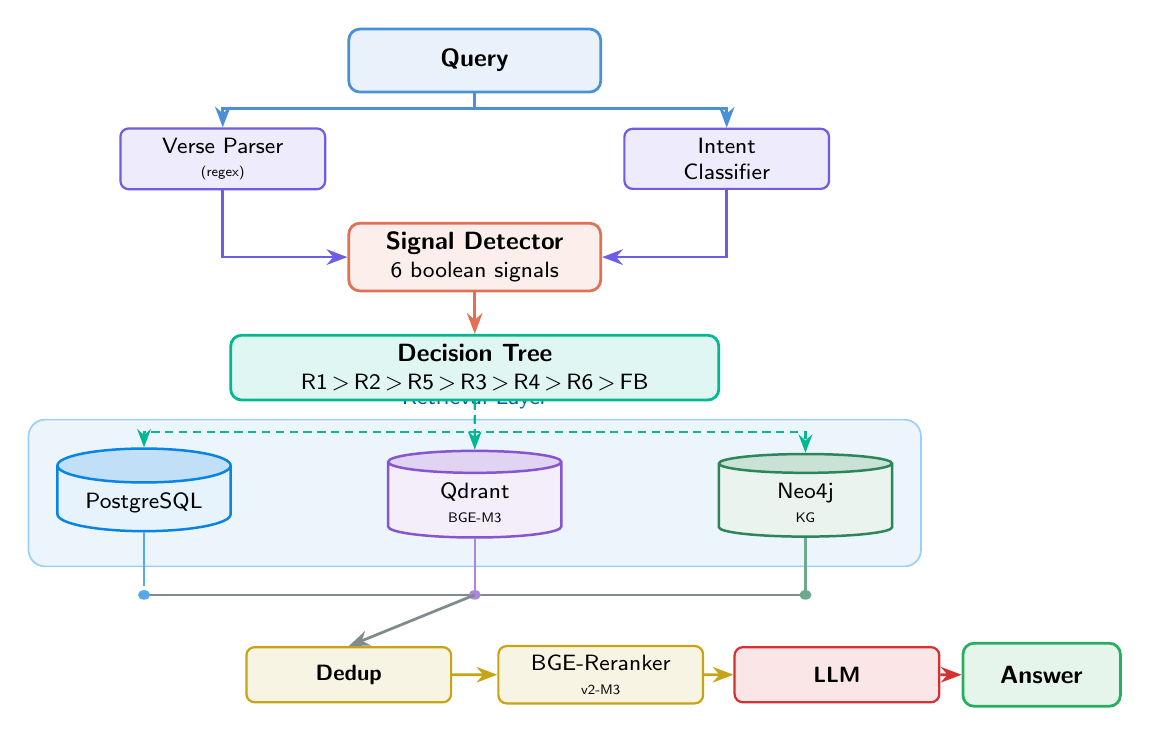
\begin{tikzpicture}[yscale=0.78,
    >=Stealth,
    block/.style={
        rectangle, rounded corners=4pt, draw=#1, fill=#1!12,
        line width=1pt, minimum height=0.8cm, minimum width=3.2cm,
        font=\sffamily\small, align=center, text=black
    },
    smallblock/.style={
        rectangle, rounded corners=3pt, draw=#1, fill=#1!12,
        line width=0.8pt, minimum height=0.7cm, minimum width=2.6cm,
        font=\sffamily\footnotesize, align=center, text=black
    },
    dbnode/.style={
        cylinder, cylinder uses custom fill, cylinder end fill=#1!25,
        cylinder body fill=#1!10, draw=#1, line width=0.9pt,
        shape border rotate=90, aspect=0.25,
        minimum height=0.9cm, minimum width=2.2cm,
        font=\sffamily\footnotesize, align=center, text=black
    },
    arr/.style={->, line width=1pt, color=#1},
    darr/.style={->, line width=0.8pt, densely dashed, color=#1},
]

% Row 1 – Query
\node[block=cQuery] (query) at (0,0) {\textbf{Query}};

% Row 2 – Verse Parser + Intent Classifier
\node[smallblock=cParse] (parser) at (-3.2,-1.6) {Verse Parser\\[-1pt]{\tiny (regex)}};
\node[smallblock=cParse] (intent) at ( 3.2,-1.6) {Intent\\Classifier};

% Row 3 – Signal Detector
\node[block=cSignal] (signal) at (0,-3.2) {\textbf{Signal Detector}\\[-1pt]{\footnotesize 6 boolean signals}};

% Row 4 – Decision Tree
\node[block=cTree, minimum width=6.2cm] (tree) at (0,-5.0)
    {\textbf{Decision Tree}\\[-1pt]
     {\footnotesize R1\,$>$\,R2\,$>$\,R5\,$>$\,R3\,$>$\,R4\,$>$\,R6\,$>$\,FB}};

% Row 5 – Databases
\node[dbnode=cDB]    (pg)     at (-4.2,-7.2) {PostgreSQL};
\node[dbnode=cDBvec] (qdrant) at ( 0.0,-7.2) {Qdrant\\[-1pt]{\tiny BGE-M3}};
\node[dbnode=cDBneo] (neo4j)  at ( 4.2,-7.2) {Neo4j\\[-1pt]{\tiny KG}};

% Row 6 – Post-retrieval pipeline
\node[smallblock=cPipe] (dedup)  at (-1.6,-10.0) {\textbf{Dedup}};
\node[smallblock=cPipe] (rerank) at ( 1.6,-10.0) {BGE-Reranker\\[-1pt]{\tiny v2-M3}};
\node[smallblock=cLLM]  (llm)    at ( 4.6,-10.0) {\textbf{LLM}};
\node[block=cAnswer, minimum width=2.0cm] (answer) at (7.2,-10.0) {\textbf{Answer}};

% Background – Retrieval Layer
\begin{scope}[on background layer]
    \node[fit=(pg)(qdrant)(neo4j),
          fill=bgDB, rounded corners=6pt,
          inner sep=10pt, draw=cDB!40, line width=0.6pt,
          label={[font=\sffamily\footnotesize\color{cDB!70!black}]
                 above:Retrieval Layer}] {};
\end{scope}

% Arrows – top section
\draw[arr=cQuery] (query.south) -- ++(0,-0.25) -| (parser.north);
\draw[arr=cQuery] (query.south) -- ++(0,-0.25) -| (intent.north);
\draw[arr=cParse] (parser.south) |- (signal.west);
\draw[arr=cParse] (intent.south) |- (signal.east);
\draw[arr=cSignal] (signal) -- (tree);

% Arrows – Decision Tree to DBs (dashed)
\draw[darr=cTree] (tree.south) -- ++(0,-0.5) -| (pg.north);
\draw[darr=cTree] (tree.south) --               (qdrant.north);
\draw[darr=cTree] (tree.south) -- ++(0,-0.5) -| (neo4j.north);

% Arrows – DBs to Dedup via bus line
\draw[line width=0.9pt, color=cDB!70]    (pg.south)     -- ++(0,-0.87);
\draw[line width=0.9pt, color=cDBvec!70] (qdrant.south) -- ++(0,-0.87);
\draw[line width=0.9pt, color=cDBneo!70] (neo4j.south)  -- ++(0,-0.87);
\draw[line width=0.9pt, color=cBus] (-4.2,-8.7) -- (4.2,-8.7);
\fill[cDB!70]    (-4.2,-8.7) circle (2.2pt);
\fill[cDBvec!70] ( 0.0,-8.7) circle (2.2pt);
\fill[cDBneo!70] ( 4.2,-8.7) circle (2.2pt);
\draw[arr=cBus, line width=1pt] (0,-8.7) -- (dedup.north);

% Arrows – post-retrieval chain
\draw[arr=cPipe] (dedup)  -- (rerank);
\draw[arr=cPipe] (rerank) -- (llm);
\draw[arr=cLLM]  (llm)    -- (answer);

\end{tikzpicture}%
}% end resizebox
\caption{Signal-driven 6-route RAG pipeline.}
\label{fig:pipeline}
\end{figure}

\subsection{Data Processing Pipeline}

The 66 books of the Traditional Chinese Bible are processed through hierarchical chunking: Book (66) $\rightarrow$ Chapter (1,189) $\rightarrow$ Pericope (2,779) $\rightarrow$ Chunk (438), with token-aware splitting (512--1024 tokens) respecting verse boundaries. CKIP Transformers \cite{ckip2021} perform Chinese NER with LLM validation, extracting 14,845 entities across 6 types (Person, Place, Event, Theme, Object, Group) linked to text via 49,668 MENTIONS edges. BGE-M3 \cite{bge2024} generates 1024-dim embeddings for 3,041 vectors stored in Qdrant.

\subsection{Triple-Database Architecture}

PostgreSQL stores structured verse/chapter/book data (100,222 records) for exact lookup. Qdrant provides dense vector search via cosine similarity over 3,041 embedding points. Neo4j maintains a knowledge graph with 19,317 nodes and 58,031 relationships across 5 edge types: MENTIONS (49,668), CONTAINS (4,406), NEXT (2,980), CROSS\_REFERENCES (912), and NEXT\_BOOK (65).

\subsection{Signal-Driven 6-Route Retrieval}

Each query undergoes regex verse parsing and LLM intent classification. A \textit{signal detector} evaluates six boolean features---verse reference, chapter reference, multi-book, multi-person, event keyword, and place name---via regex and dictionary matching against knowledge graph entity lists. A priority-ordered decision tree (Table~\ref{tab:routes}) routes queries: R1 performs direct SQL verse lookup; R2 combines SQL chapter filtering with semantic search; R3/R4/R6 launch parallel graph traversals (Person/Event/Place$\rightarrow$MENTIONS) alongside semantic and SQL retrieval; R5 uses semantic seed passages to feed CROSS\_REFERENCES traversal; the Fallback defaults to pure semantic search. All routes except R1 undergo deduplication and BGE-Reranker-v2-M3 \cite{bge2024} reranking. A pluggable LLM factory supports multiple providers with identical evidence-first prompting; the LLM also performs intent classification, so model switching can affect routing (Section~IV).

\begin{table}[h]
\centering
\caption{Signal-Driven Route Overview and Engine Weight Matrix}
\label{tab:routes}
\footnotesize
\begin{tabular}{@{}llcccc@{}}
\toprule
Route & Signal & SQL & Sem. & Graph & XRef \\
\midrule
R1 & book+ch:v     & 1.00 & ---  & ---  & --- \\
R2 & book+ch       & 0.90 & 0.60 & ---  & --- \\
R3 & $\geq$2 persons  & 0.50 & 0.70 & 0.90 & --- \\
R4 & event kw      & 0.50 & 0.70 & 0.85 & --- \\
R5 & $\geq$2 books/xref & 0.40 & 0.65 & 0.75 & 0.85 \\
R6 & place         & 0.50 & 0.70 & 0.85 & --- \\
FB & (else)        & ---  & 1.00 & ---  & --- \\
\bottomrule
\end{tabular}
\end{table}

\section{Experiments}

\textbf{Setup.} We curated 100 questions across 5 types (20 each): VERSE\_LOOKUP, TOPIC, PERSON, EVENT, and GENERAL, mapped to routes R1--R5 respectively. We compare Claude Haiku 4.5 (commercial API) \cite{anthropic2024} against Gemma 3 4B (local Ollama) \cite{gemma2025} sharing the same retrieval codebase (temperature=0.1, top\_k=5). We employ 19 metrics in 4 categories: retrieval (7), reference-based (5), semantic (1), and LLM-judged (6, via RAGAS \cite{ragas2024}).

\begin{table}[h]
\centering
\caption{Overall Performance Comparison (Selected Metrics)}
\label{tab:metrics}
\footnotesize
\begin{tabular}{@{}llccc@{}}
\toprule
Category & Metric & Claude & Gemma & $\Delta$ \\
\midrule
\textit{Retrieval} & Hit Rate      & 0.790 & 0.820 & +0.030 \\
                    & Recall@5      & 0.746 & 0.761 & +0.015 \\
                    & MRR           & 0.753 & 0.782 & +0.029 \\
\midrule
\textit{LLM Judge} & Faithfulness  & 0.887 & 0.849 & $-$0.039 \\
                    & Ans.\ Relevancy & 0.592 & 0.658 & +0.066 \\
                    & Ctx.\ Recall  & 0.678 & 0.712 & +0.034 \\
                    & Ans.\ Correctness & 0.572 & 0.557 & $-$0.015 \\
\midrule
\textit{Semantic}   & Similarity    & 0.738 & 0.729 & $-$0.009 \\
\midrule
\textit{Ref-based}  & BERTScore     & 0.663 & 0.685 & +0.022 \\
\bottomrule
\end{tabular}
\end{table}

\begin{table}[h]
\centering
\caption{Answer Correctness by Question Type (Route)}
\label{tab:pertype}
\footnotesize
\begin{tabular}{@{}lccc@{}}
\toprule
Type (Route) & Claude & Gemma & $\Delta$ \\
\midrule
VERSE (R1)   & 0.841 & 0.886 & +0.044 \\
TOPIC (R2)   & 0.657 & 0.622 & $-$0.036 \\
PERSON (R3)  & 0.440 & 0.418 & $-$0.022 \\
EVENT (R4)   & 0.457 & 0.440 & $-$0.017 \\
GENERAL (R5) & 0.416 & 0.370 & $-$0.047 \\
\bottomrule
\end{tabular}
\end{table}

\section{Results and Discussion}

\textit{Finding 1: Complementary Model Strengths.}
Table~\ref{tab:metrics} shows that 9 of 12 generation metrics differ by less than 4 percentage points. The models exhibit complementary strengths: Claude achieves higher faithfulness (0.887 vs.\ 0.849), indicating stricter citation behavior, while Gemma leads on answer relevancy (0.658 vs.\ 0.592), suggesting more comprehensive responses. Retrieval metrics are identical for signal-deterministic routes (R1, R2) but diverge slightly for R3--R5, where LLM-dependent intent classification affects entity extraction and thus graph traversal inputs. This confirms that when high-quality context is provided, model differences manifest as generation style rather than fundamental quality gaps.

\textit{Finding 2: Route-Specific Analysis.}
Table~\ref{tab:pertype} reveals clear route-dependent patterns. VERSE (R1) scores highest (0.841/0.886) because SQL direct match provides exact evidence; Gemma's stronger BLEU (0.547 vs.\ 0.173) on this route suggests closer lexical alignment with reference answers. GENERAL (R5) scores lowest (0.416/0.370) as the cross-reference path---the most complex 4-engine route---faces sparser CROSS\_REFERENCES edges (912 total). EVENT (R4) also challenges both models (0.457/0.440) since multi-chapter narratives strain fixed-window chunking. Claude leads on TOPIC and GENERAL; Gemma leads on VERSE, indicating complementary biases tied to route complexity.

\textit{Finding 3: Cost-Quality Tradeoff.}
Gemma 3 4B runs locally with zero API cost and full data privacy. Neither model dominates overall, making the local option viable for production. The key investment shifts from model scale to retrieval infrastructure: RAG compensates for smaller models' limited domain knowledge by supplying structured evidence. Low ROUGE ($<$0.03) with moderate semantic similarity (0.738/0.729) confirms paraphrased but accurate generation driven by retrieval quality.

\section{Conclusion}

We presented a signal-driven Graph RAG for Traditional Chinese Bible QA with a 6-route decision-tree router over PostgreSQL, Qdrant, and Neo4j. A local Gemma 3 4B matches Claude Haiku 4.5 on 9 of 12 metrics within 4 percentage points, confirming that retrieval design---not model scale---primarily determines domain QA quality while eliminating API costs. Future work includes hybrid dense-sparse retrieval \cite{robertson2009}, adaptive route weights, and multilingual evaluation.

\begin{thebibliography}{10}
\bibitem{lewis2020} P.~Lewis \textit{et al.}, ``Retrieval-augmented generation for knowledge-intensive NLP tasks,'' \textit{NeurIPS}, 2020.
\bibitem{edge2024} D.~Edge \textit{et al.}, ``From local to global: A graph RAG approach to query-focused summarization,'' \textit{arXiv:2404.16130}, 2024.
\bibitem{gao2024} Y.~Gao \textit{et al.}, ``Retrieval-augmented generation for large language models: A survey,'' \textit{arXiv:2312.10997}, 2024.
\bibitem{bge2024} J.~Chen \textit{et al.}, ``BGE M3-embedding: Multi-lingual, multi-functionality, multi-granularity text embeddings through self-knowledge distillation,'' \textit{arXiv:2402.03216}, 2024.
\bibitem{ragas2024} S.~Es \textit{et al.}, ``RAGAS: Automated evaluation of retrieval augmented generation,'' \textit{arXiv:2309.15217}, 2024.
\bibitem{gemma2025} Google DeepMind, ``Gemma 3 technical report,'' \textit{arXiv:2503.19786}, 2025.
\bibitem{anthropic2024} Anthropic, ``The Claude model family,'' 2024.
\bibitem{ckip2021} W.-Y.~Ma and K.-J.~Chen, ``CKIP Transformers: An NLP toolkit for traditional Chinese,'' in \textit{Proc. ROCLING}, 2021.
\bibitem{karpukhin2020} V.~Karpukhin \textit{et al.}, ``Dense passage retrieval for open-domain question answering,'' \textit{EMNLP}, 2020.
\bibitem{robertson2009} S.~Robertson and H.~Zaragoza, ``The probabilistic relevance framework: BM25 and beyond,'' \textit{Found. Trends Inf. Retr.}, 2009.
\end{thebibliography}

\end{document}
